\section*{Pulse-amplitude modulation (PAM)}

La PAM nel caso generico è detta anche \( M \)-PAM o PAM \( M \)-aria dove con \( M \) si indica il numero di simboli presenti nell'alfabeto \( A_s \).

\begin{center}
    \begin{tikzpicture}
        \node (s) at (0,0) {\(x[k]\)};
        \node[block] (encoder) at (3,0) {\(p(t)\)};
        \node (r) at (6,0) {\(s(t)\)};

        \draw[->] (s) -- (encoder);
        \draw[->] (encoder) -- (r);
    \end{tikzpicture}
\end{center}

Proprietà che definiscono una \( M \)-PAM:

\begin{enumerate}
    \item \( s(t) \coloneqq \sum_{k=-\infty}^{+\infty} x[k]\cdot p(t - kT_s) \)
    \item Gli \( M \) valori \( (M \geq 2) \) che costituiscono l'alfabeto \( A_s = \{ \alpha_1, \alpha_2, \ldots, \alpha_M \} \) sono definiti come:
          \[ \alpha_i = 2i - 1 - M, \quad i = 1, 2, \ldots, M \]
\end{enumerate}

Esempio:

\( M=4 \) $\Rightarrow$ \( \alpha_1 = -3, \alpha_2 = -1, \alpha_3 = 1, \alpha_4 = 3 \)

\begin{center}
    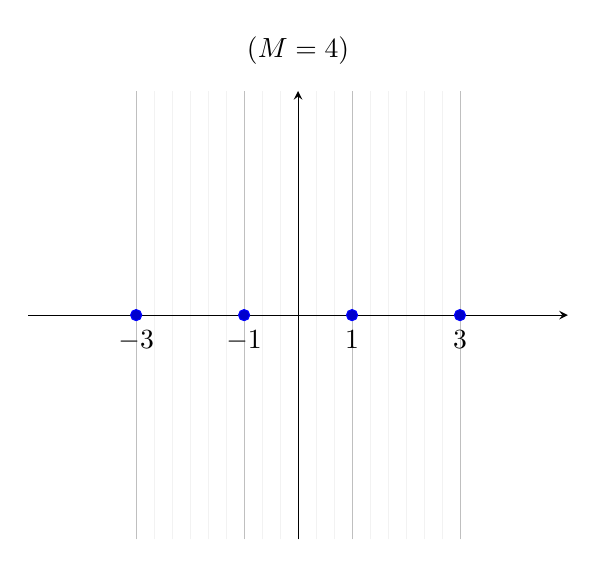
\begin{tikzpicture}
        \begin{axis}[
                title={\( (M=4) \)},
                xlabel={},
                ylabel={},
                xmin=-5, xmax=5,
                ymin=-4, ymax=4,
                grid=both,
                grid style={line width=.1pt, draw=gray!10},
                major grid style={line width=.2pt,draw=gray!50},
                minor tick num=5,
                axis lines=middle,
                minor tick style={draw=none},
                xtick={-3, -1, 1, 3},
                ytick=\empty,
            ]

            \addplot+[only marks] coordinates {
                    (-3, 0)
                    (-1, 0)
                    (1, 0)
                    (3, 0)
                };
        \end{axis}
    \end{tikzpicture}
\end{center}
\[
    E_s(i) = \int_{-\infty}^{+\infty} s_i^2(t) \, dt =  \int_{-\infty}^{+\infty} \alpha_i^2 \cdot p^2(t - kT_s) \, dt = \int_{-\infty}^{+\infty} (2i - 1 - M)^2 p^2(t) \, dt = (2i - 1 - M)^2 E_p
\]

Per \( M \) pari si ha \( A_s = \{ \pm 1, \pm 3, \ldots, \pm (M-1) \} \)

Per \( M \) dispari si ha \( A_s = \{ 0, \pm 2, \pm 4, \ldots, \pm (M-1) \} \)

I formati M-PAM di pi\`u largo impiego sono quelli dove $M$ è una potenza di 2.

Esempio:

$4$-PAM

sequenza = $\left\{ \begin{array}{l}
        x[-2] = -1, \\
        x[-1] = 1,  \\
        x[0] = -3,  \\
        x[1] = 1,   \\
        x[2] = 3    \\
    \end{array} \right.$

$p(t) = \text{rect}\left(\frac{t - T_s/2}{T_s}\right)$

\begin{center}
    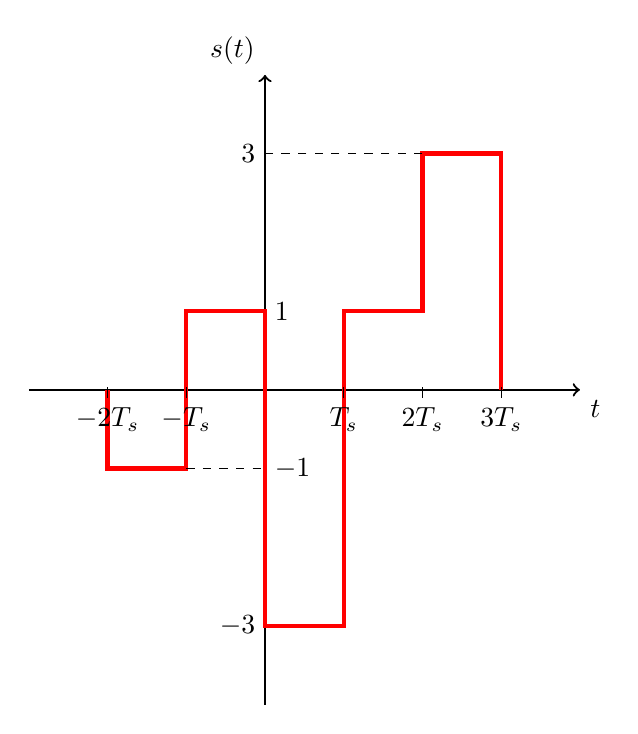
\begin{tikzpicture}
        % Assi
        \draw[thick,->] (-3,0) -- (4,0) node[anchor=north west] {$t$};
        \draw[thick,->] (0,-4) -- (0,4) node[anchor=south east] {$s(t)$};

        % Grafico a gradini
        \draw[ultra thick, red] (-2,0) -- (-2,-1) -- (-1,-1) -- (-1,1) -- (0,1) -- (0,-3) -- (1,-3) -- (1,1) -- (2,1) -- (2,3) -- (3,3) -- (3,0);

        % Tacche e etichette sull'asse delle x
        \foreach \x in {-2,2,3}
        \draw (\x cm,1pt) -- (\x cm,-3pt)
        node[anchor=north] {$\x T_s$};

        \draw (-1 cm,1pt) -- (-1 cm,-3pt)
        node[anchor=north] {$-T_s$};
        \draw (1 cm,1pt) -- (1 cm,-3pt)
        node[anchor=north] {$T_s$};

        % Linee tratteggiate
        \draw[dashed] (-1,-1) -- (0,-1);
        \draw[dashed] (2,3) -- (0,3);

        % Etichette
        \node at (0,1) [right] {$1$};
        \node at (0,-1) [right] {$-1$};
        \node at (0,3) [left] {$3$};
        \node at (0,-3) [left] {$-3$};
    \end{tikzpicture}
\end{center}

\subsection*{Proprietà derivate della M-PAM}
\begin{enumerate}
    \item Il valor medio di \( s(t) \) è zero per ogni \( t \):
          \begin{equation*}
              \mathbb{E}\left[ s(t) \right] = 0 \quad \forall t
          \end{equation*}
          \begin{equation*}
              \mathbb{E} \left[ \sum_{k=-\infty}^{+\infty} x[k] \ p(t-kT_s) \right] = \sum_{k=-\infty}^{+\infty} \mathbb{E}\left[x[k]\right]\ p(t-kT_s) = 0
          \end{equation*}
          \begin{equation*}
              \mathbb{E}\left[x[k]\right] = \frac{1}{M} \sum_{i=1}^{M} \alpha_i \mathbb{P}\{\alpha_i\} = \frac{1}{M} \sum_{i=1}^{M} (2i - 1 - M)
          \end{equation*}
          \begin{equation*}
              = \frac{2}{M} \sum_{i=1}^{M} i - 1 - M = \frac{2}{M} \frac{M(M+1)}{2} - (M+1) = 0
          \end{equation*}

    \item La densità spettrale di potenza invece è: \( S_s(f) \):
          \begin{equation*}
              S_s(f) = \frac{1}{T_s} S_x(f) \ |P(f)|^2
          \end{equation*}
          \begin{equation*}
              \text{dove } \sigma_x^2 = \mathbb{E}\left[ x\left[k\right]^2 \right] = \frac{(M-1)(M+1)}{3}
          \end{equation*}
\end{enumerate}

\[
    R_s(t,\tau) = \mathbb{E}[s(t) \ s^*(t-\tau)]
\]
\[
    = \mathbb{E} \left[ \sum_{n=-\infty}^{+\infty} x\left[n\right] p(t - nT_s) \sum_{k=-\infty}^{+\infty} x^*\left[k\right] p^*(t - \tau - kT_s) \right]
\]
\[
    = \sum_{n=-\infty}^{+\infty} \sum_{k=-\infty}^{+\infty} \mathbb{E}[x\left[n\right] x^*\left[k\right]] \cdot p(t - nT_s) \cdot p^*(t - \tau - kT_s)
\]
\[
    = \sum_{n=-\infty}^{+\infty} \sum_{k=-\infty}^{+\infty} R_x\left[n-k\right] \cdot p(t - nT_s) \cdot p^*(t - \tau - kT_s)
\]

Imponendo \( n-k = m \) abbiamo che \( k = n-m \), quindi:

\[
    = \sum_{m=-\infty}^{+\infty} R_x[m] \sum_{n=-\infty}^{+\infty} p(t - nT_s) \cdot p^*(t - \tau - nT_s + mT_s)
\]

\paragraph*{Autocorrelazione media}

La funzione di autocorrelazione media \( \overline{R}_s(\tau) \) è:
\begin{align*}
    \overline{R}_s(\tau) & = \lim_{T\to\infty} \frac{1}{T} \int_{-\frac{T}{2}}^{\frac{T}{2}} R_s(t, \tau) dt                                                                   \\
    \overline{R}_s(\tau) & = \frac{1}{T_0} \int_{-\frac{T_0}{2}}^{\frac{T_0}{2}} R_s(t,\tau)dt \quad \text{se} \quad R_s(t,\tau) \quad \text{è periodico in} \quad t           \\
    \overline{R}_s(\tau) & = \sum_{m=-\infty}^{\infty} R_x[m] \frac{1}{T_s} \sum_{n=-\infty}^{\infty} \int_{-\frac{T_s}{2}}^{\frac{T_s}{2}} p(t-nT_s)p^*(t-\tau-nT_s+mT_s)dt   \\
                         & = \sum_{m=-\infty}^{\infty} R_x[m] \frac{1}{T_s} \sum_{n=-\infty}^{\infty}\int_{-\frac{T_s}{2}+nT_s}^{\frac{T_s}{2}+nT_s} p(t')p^*(t'-\tau+mT_s)dt' \\
                         & = \sum_{m=-\infty}^{\infty} R_x[m] \frac{1}{T_s} \int_{-\infty}^{\infty} p(t')p^*(t'-\tau+mT_s)dt'                                                  \\
                         & = \sum_{m=-\infty}^{\infty} R_x[m] \frac{1}{T_s} \int_{-\infty}^{\infty} P(f)[P(f)e^{-j2\pi f\tau}e^{j2\pi fmT_s}]^*df                              \\
                         & = \int_{-\infty}^{\infty} P(f)P^*(f)\frac{1}{T_s} \sum_{m=-\infty}^{\infty} R_x[m] e^{-j2\pi fmT_s}e^{j2\pi f\tau}df                                \\
                         & = \frac{1}{T_s} \int_{-\infty}^{\infty} |P(f)|^2 S_x(f)e^{j2\pi f\tau}df
\end{align*}


\[
    \overline{R}_s(\tau) = \frac{1}{T_s} TCF^{-1} \left[ |P(f)|^2 S_x(f) \right]
\]
\[
    \Rightarrow S_s(f) = \frac{1}{T_s} S_x(f) |P(f)|^2
\]

Nel caso in cui:
\begin{enumerate}
    \item $\mathbb{E} [ x[n] ] = 0$
    \item $R_x[m] = \sigma_x^2 \delta[m]$
\end{enumerate}

Si ha che:
\[
    S_s(f) = \frac{\sigma_x^2}{T_s} |P(f)|^2
\]

In questo caso la $B_T$ coincide con quella del sagomatore $P(f)$.

Calcolo di $\sigma_x^2$:
\[
    \sigma_x^2 = \mathbb{E} \left[ (x - \mu_x)^2 \right] = \int_{-\infty}^{\infty} (x - \mu_x)^2 f_x(x) dx
\]
\[
    = \frac{1}{M} \sum_{i=1}^{M} (2i - 1 - M)^2
\]
\[
    = \frac{1}{M} \left[ 2 \sum_{i=1}^{M} i^2 + (1+M)^2 M - 4(1+M) \sum_{i=1}^{M} i \right]
\]

Sfruttando i seguenti risultati noti:
\[
    \sum_{i=1}^{n} i^2 = \frac{n(n+1)(2n+1)}{6}, \quad \sum_{i=1}^{n} i = \frac{n(n+1)}{2}
\]

Si ottiene:
\[
    \sigma_x^2 = \frac{M^2 - 1}{3}
\]

\[
    P_s = \frac{\sigma_x^2 E_p}{T_s} = \frac{M^2 - 1}{3} \frac{E_p}{T_s}
\]

\paragraph*{Efficienza Spettrale di una M-PAM}
\[
    \beta = \frac{R_b}{B_T} = \frac{\log_2 M}{T_s B_P}
\]
essendo \( B_T = B_P \),

L'efficienza spettrale aumenta con l'aumentare del numero di livelli. Sfortunatamente, come verrà dimostrato più avanti, l'efficienza in potenza diminuisce all'aumentare di \( M \).

\subsection*{PAM Binaria o BPSK (Binary Phase Shift Keying)}


\[
    s(t) = \sum_{k=-\infty}^{\infty} x[n] p(t - kT_s)
\]
con \( x[n] \in A_s = \{\pm 1\} \) (M = 2)

\[
    \Rightarrow T_B = T_s \quad (\log_2 2 = 1)
\]

Esempio con \( p(t) = \text{rect}\left(\frac{t-T_s/2}{T_s}\right) \)

% Drawing the binary PAM signal
\begin{center}

    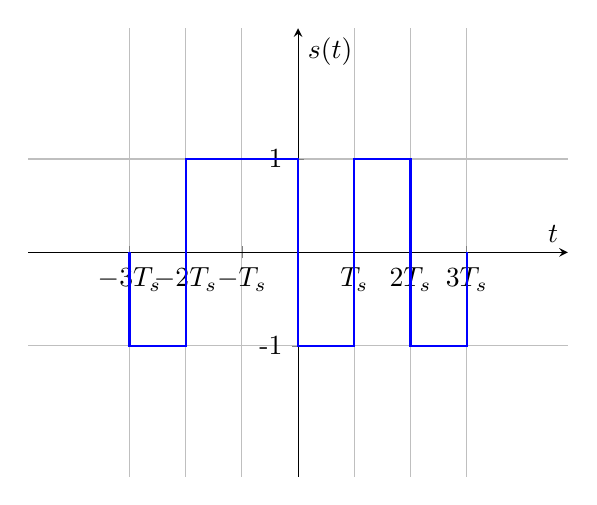
\begin{tikzpicture}
        \begin{axis}[
                xlabel = \( t \),
                ylabel = \( s(t) \),
                xtick={-3, -2, ..., 3},
                ytick={-1, 1},
                yticklabels={-1, 1},
                xticklabels={\(-3T_s\), \(-2T_s\), \(-T_s\), 0, \(T_s\), \(2T_s\), \(3T_s\)},
                ymin=-2, ymax=2,
                xmin=-4, xmax=4,
                axis lines=middle,
                enlargelimits=true,
                clip=false,
                grid=both
            ]
            \addplot+[const plot, no marks, thick] coordinates {(-3, 0) (-3,-1) (-2,-1) (-2,1) (0,-1) (1,1) (2,-1) (3,0)};
        \end{axis}
    \end{tikzpicture}
\end{center}
\[
    \text{Segnale PAM binario (o BPSK)}
\]

Il PAM Binario è un formato equiprobabile

% Energy calculation
\[
    E_{s_1} = \int_{-\infty}^{\infty} s_1^2(t) dt = \int_{-\infty}^{\infty} \left( +1 \right)^2 p^2(t) dt =  \int_{-\infty}^{\infty} \left( -1 \right)^2 p^2(t) dt = \int_{-\infty}^{\infty}  p^2(t) dt  = E_{s_2}
\]

\[
    E_{s_1} = E_{s_2} = \int_{-\infty}^{\infty} p^2(t) dt = E_p
\]

% Drawing the constellation diagram
\begin{center}

    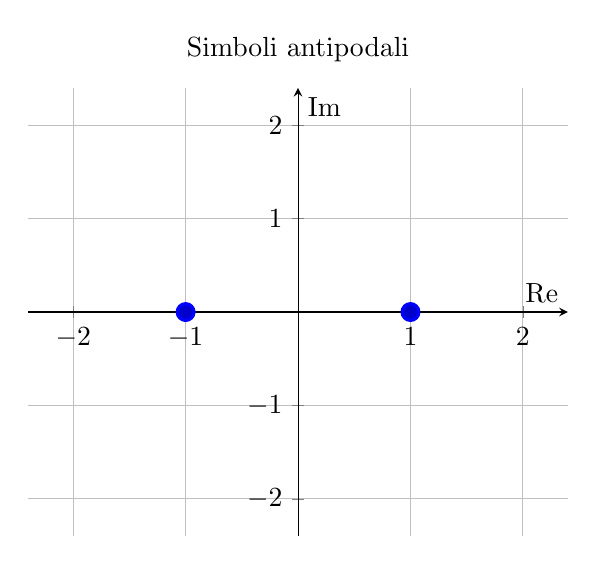
\begin{tikzpicture}
        \begin{axis}[
                title={Simboli antipodali},
                xlabel={Re},
                ylabel={Im},
                xmin=-2, xmax=2,
                ymin=-2, ymax=2,
                grid=both,
                axis lines=middle,
                enlargelimits=true
            ]
            \addplot+[only marks, mark size=3, very thick] coordinates {(1, 0) (-1, 0)};
            \node at (axis cs:1,0) [anchor=west] {};
            \node at (axis cs:-1,0) [anchor=east] {};
        \end{axis}
    \end{tikzpicture}
\end{center}



\begin{enumerate}
    \item $\mathbb{E}\left[s(t)\right] = \dfrac{1}{2} \sum_{k=-\infty}^{+\infty} \mathbb{E}[x_k] p(t-kT_s)
              = \sum_{k=-\infty}^{+\infty} \left(\dfrac{1}{2} (+1) + \dfrac{1}{2} (-1)\right) p(t-kT_s) = 0 \quad \text{se i simboli sono equiprobabili}$

    \item $S_s(t) = \dfrac{1}{T_b} |P(f)|^2 \quad \text{Densità spettrale di potenza}$

    \item $P_s = \dfrac{E_p}{T_b} \quad \text{Potenza media}$

    \item $B_T = B_P \quad \text{Banda}$

    \item $M_P = \dfrac{1}{T_bB_p}$
\end{enumerate}

\paragraph{Segnalazione ON-OFF}

È un tipo di PAM binaria con simboli appartenenti ad $A_s = \{0, 1\}$

e impulsi rettangolari  $p(t) = \text{rect}\left(\dfrac{t-T_b/2}{T_b}\right)$

\[
    s(t) = \sum_{k=-\infty}^{+\infty} x\left[k\right] \text{rect}\left(\dfrac{t-T_b/2-kT_b}{T_b}\right)
\]

\[
    \begin{cases}
        S_1(t) = 0                                            & \Rightarrow E_{S_1} = 0   \\
        S_2(t) = \text{rect}\left(\dfrac{t-T_b/2}{T_b}\right) & \Rightarrow E_{S_2} = T_b
    \end{cases}
\]


\begin{itemize}
    \item $
              \mathbb{E}[S(t)] = \sum_{k=-\infty}^{+\infty} \mathbb{E}[x[k]] p(t-kT_b) = \dfrac{1}{2}$
    \item $
              E_s = \dfrac{1}{2}E_{S_1} + \dfrac{1}{2}E_{S_2} = \dfrac{T_b}{2}
          $
    \item
          $
              P_s = \dfrac{E_s}{T_b} = \dfrac{1}{2}$
    \item $R_x[m] = C_x[m] + {\eta}_x^2 = \frac{1}{4} {\delta}[m] + \frac{1}{4}$

    \item $S_x(f) = TFS\left[ R_x[m] \right] = \frac{1}{4} + \frac{1}{4T_b} \sum_{m=-\infty}^{\infty} \delta\left(f - \frac{m}{T_b}\right)$
    \item $S_s(f) = \frac{1}{T_b} S_x(f)|P(f)|^2 = \frac{1}{T_b} \left( \frac{1}{4} + \frac{1}{4T_b} \delta(f) \right) T_b^2 \operatorname{sinc}^2(T_b f) = \frac{T_b}{4} \left( 1 + \frac{\delta(f)}{T_b} \right)\operatorname{sinc}^2(T_b f)$

    \item ${\eta}_b = \frac{\log_2{2}}{T_b B_p} = 2 \quad \text{e} \quad B_p = \frac{1}{2T_b} \text{ per la sinc}$
\end{itemize}



% Considerazioni
\subsection*{Considerazioni}
\begin{enumerate}
    \item L'efficienza spettrale della modulazione on-off è unitaria come nel caso della 2-PAM.
    \item Essendo la modulazione on-off di tipo unipolare (solo a valori positivi) questa può essere utilizzata su canali di comunicazione che, per loro natura, non possono sovrapporre segnali bipolari.
    \item La densità spettrale della on-off presenta un impulso di dirac nell'origine delle frequenze (alla continua) per cui il canale di trasmissione deve avere una risposta in frequenza che non sia nulla nell'origine.
\end{enumerate}
